\chapter{User guide}

\section{Setting up ESP32 toolkit}

This is the guide to install all the necessary software to execute the FreeRTOS IoT monitoring demo found in the repository: https://github.com/C4ES-PoliTO/FreeRTOS-Monitoring
\\~\\
This installation guide is meant to be followed using a \href{https://docs.espressif.com/projects/esp-idf/en/latest/esp32/get-started/linux-macos-setup.html}{\textbf{Linux}} operating system (Ubuntu or Debian), for information on running on other operating systems, take a look at: \href{https://docs.espressif.com/projects/esp-idf/en/latest/esp32/get-started/windows-setup.html}{\textbf{Windows}} , \href{https://docs.espressif.com/projects/esp-idf/en/latest/esp32/get-started/linux-macos-setup.html}{\textbf{MacOS}}.
\\~\\
\textbf{Setting up the ESP32 environment:}
\\
\begin{itemize}
    \item Command to install the required packages:
    \begin{verbatim}
    sudo apt-get install git wget flex bison gperf python3 python3-venv cmake 
    ninja-build ccache libffi-dev libssl-dev dfu-util libusb-1.0-0
    \end{verbatim}

    Note: cmake version 3.5 or higher is required, to check the version run: cmake --version
    
    \item Proceed by cloning the software libraries provided by ESP-IDF repository, to do this, create a parent folder and run:
    \begin{verbatim}
    mkdir -p ~/esp
    cd ~/esp
    git clone -b v4.4.1 --recursive https://github.com/espressif/esp-idf.git
    \end{verbatim}

    
    
    \item Update python:
    \begin{verbatim}
    sudo apt update
    sudo apt install python3
    sudo apt-get install python3-venv
    sudo apt intall pip
    \end{verbatim}


    \item Aside from the ESP-IDF, you also need to install the tools used by ESP-IDF, such as the compiler, debugger, Python packages, etc, for projects supporting ESP32:
    \begin{verbatim}
    cd ~/esp/esp-idf
    ./install.sh esp32
    \end{verbatim}

    
    \item The installed tools are not yet added to the PATH environment variable. To make the tools usable from the command line, some environment variables must be set. ESP-IDF provides another script which does that.\\
    
    In the terminal where you are going to use ESP-IDF, run:
    \begin{verbatim}
    . $HOME/esp/esp-idf/export.sh 
    \end{verbatim}
    
    Note the space between the leading dot and the path!

\end{itemize}

\textbf{Running an ESP32 project:}

\begin{itemize}
    \item Clone project files 
    \begin{verbatim}
    cd ~
    git clone https://github.com/C4ES-PoliTO/FreeRTOS-Monitoring.git
    \end{verbatim}

    
    \item \textbf{Navigate} to the project directory, set ESP32 and run the project configuration utility menuconfig:
    \begin{verbatim}
    cd FreeRTOS-Monitoring/Source_code/esp32_leaf_node
    idf.py set-target esp32
    idf.py menuconfig
    menuconfig->Component config->FreeRTOS->Enable FreeRTOS trace facility
    menuconfig->Example Configuration Connection >WiFi SSID  
    menuconfig->Example Configuration Connection >WiFi Password
    \end{verbatim}

    Trace facibility for FreeRTOS needs to be enabled, set WiFi credentials, for the leaf node, use the ones provided by the gateway.\\
    
    After opening a new project, you should first \textbf{set the target}. Note that existing builds and configurations in the project, if any, will be cleared and initialized in this process. The target may be saved in the environment variable to skip this step at all.
    
    \item \textbf{To build the project:}
    \begin{verbatim}
    idf.py build
    \end{verbatim}

    If there are no errors, the build will finish by generating the firmware binary .bin files.

    \item \textbf{Flash} the binaries that you just built (bootloader.bin, partition-table.bin and project.bin) onto your ESP32 board by running:
    \begin{verbatim}
        idf.py -p PORT [-b BAUD] flash
    \end{verbatim}
    
    Replace PORT with your ESP32 board’s serial port name. Similar to /dev/ttyXXX

    Note: For ESP32 board, you will need to press the BOOT button on the board after executing the previous command.\\
    
    If there are no issues by the end of the flash process, the board will reboot and start up the “project.bin” application.
    If you’d like to use the Eclipse or VS Code IDE instead of running idf.py, check out the \hyperlink{https://docs.espressif.com/projects/esp-idf/en/latest/esp32/get-started/eclipse-setup.html}{Eclipse guide}, \hyperlink{https://docs.espressif.com/projects/esp-idf/en/latest/esp32/get-started/vscode-setup.html}{VS Code guide}.\\
    
    \item \textbf{Monitor the output:}\\
    To check if “project” is indeed running, type idf.py -p PORT monitor (Do not forget to replace PORT with your serial port name).
    
\end{itemize}

The instructions that are explained in this document are also available \hyperlink{https://docs.espressif.com/projects/esp-idf/en/latest/esp32/get-started/linux-macos-setup.html}{\textbf{here}}, where more information can be found, regarding different errors or suggestions that are interesting for the correct installation of the esp32 development kit. 

\section{Configuring demo}

Several parameters can be configured in the demo project, the user can choose to modify these to alter the system's behaviour.

\subsection{Central node}

\begin{figure}[H]
\centering
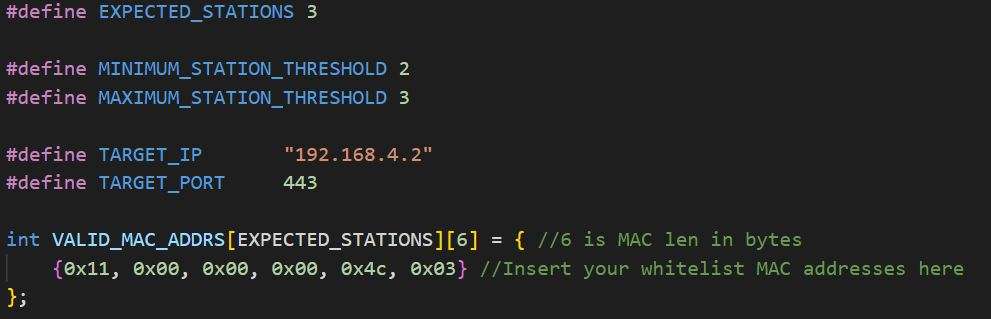
\includegraphics[width=.9\linewidth]{images/router_monitoring_params.JPG}
\caption{Parameters found in "router\_monitoring.h"}
\label{fig:router_monitoring_params}
\end{figure}

In figure \ref{fig:router_monitoring_params} we can observe the parameters that alter the behaviour of the monitoring behaviour, these are the number of expected stations, the minimum and maximum thresholds to alert the server, the IP and Port of the server that will collect the info and the whitelisted MAC addresses.
\\~\\
By default, the Wi-Fi network created by the central node is called "ESP32\_NAT\_Router" and has no password, this can be changed following the steps described \hyperlink{https://github.com/martin-ger/esp32_nat_router}{here}.

The following configuration must be done on the menuconfig

\begin{verbatim}
    menuconfig > Serial Flash Config > Flash size > 4Mb
\end{verbatim}


\subsection{Leaf node}
The leaf node offers two different configuration aspects, the first can be found in the file "sdkconfig" inside the leaf node folder, there the user can change the \textbf{CONFIG\_EXAMPLE\_WIFI\_SSID} and the \textbf{CONFIG\_EXAMPLE\_WIFI\_PASSWORD} to correspond to the ones in the central node configuration.
\\~\\
The other parameters are related to the monitoring task, and can be found in the file "taskMonitor.h". They are; the number of tasks threshold to raise an alert, the task monitoring priority and the monitoring task id which the server will recieve.



\subsection{Monitoring server}
To launch the monitoring server "upd\_server.py" found in both "esp32\_nat\_router" and "esp32\_leaf\_node" the user needs to simply navigate to any of these folders and execute the following command in the Windows/Linux terminals:

\begin{verbatim}
    python udp_server.py
\end{verbatim}

Then the server will start outputting to the console the messages that it receives.


